
\documentclass[12pt]{article}
\usepackage{amsmath}
\usepackage{times}
\usepackage{graphicx}
\usepackage{color}
\usepackage{multirow}
%
\usepackage[authoryear]{natbib}
%
\usepackage{rotating}
\usepackage{bbm}
\usepackage{latexsym}
%\DeclareGraphicsExtensions{.eps,.png}
%
\interfootnotelinepenalty=10000
%
\renewcommand{\thesubsubsection}{\arabic{section}.\arabic{subsubsection}}
\newcommand{\myparagraph}[1]{\ \\{\em #1}.\ \ }
\newcommand{\citepaltt}[1]{\citepauthor{#1},\citepyear{#1}}
\newcommand{\myycite}[1]{\citepp{#1}}

% Different font in captions
\newcommand{\captionfonts}{\normalsize}



\renewcommand{\thefootnote}{\normalsize \arabic{footnote}} 	

\newcommand{\ms}{\mbox{\,ms}}
\newcommand{\mV}{\mbox{\,mV}}
\newcommand{\s}{\mbox{\,s}}

\renewcommand{\u}{\mathbf{u}}
\renewcommand{\v}{\mathbf{v}}

\usepackage{amssymb}
\usepackage{tikz}
\usetikzlibrary{positioning}
\usetikzlibrary{arrows}

\usepackage[paperheight=4.5in,paperwidth=5in,margin=1in,heightrounded]{geometry}


\begin{document}
\thispagestyle{empty}

\begin{center}
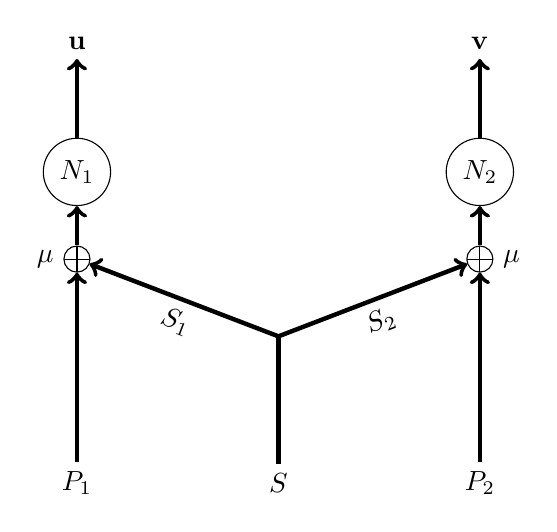
\begin{tikzpicture}[cross/.style={path picture={ 
  \draw[black] (path picture bounding box.south) -- (path picture
  bounding box.north) (path picture bounding box.west) -- (path
  picture bounding box.east); }}] \node (neuron1) at (0,0)
  [circle,draw] {$N_1$}; \node (middle)[right = 2cm of neuron1]{};
  \node (neuron2) [circle, right = 2cm of middle,draw] {$N_2$}; \node
  (a)[below = 1.5cm of neuron1]{}; \node (b)[below = 1.84cm of
    middle]{}; \node (c)[below = 1.5cm of neuron2]{};

\node (mu1)[circle,cross,below  = 0.5cm of neuron1,draw]{};
\node (mu2)[circle,cross,below  = 0.5cm of neuron2,draw]{};
\node (mumu1)[left = 0.0cm of mu1]{$\mu$};
\node (mumu2)[right = 0.0cm of mu2]{$\mu$};


\draw [ultra thick,->] (mu1)--(neuron1);
\draw [ultra thick,->] (mu2)--(neuron2);


\draw [ultra thick,->](b.center)--(mu1) node(s1)[midway, below, sloped]{$S_1$};
\draw [ultra thick,->](b.center)--(mu2) node(s2)[midway, below, sloped]{$S_2$};
\node(p1) [below=1.5cm of a]{$P_1$};
\node(s) [below=1.5cm of b]{$S$};
\node(p2) [below=1.5cm of c]{$P_2$};
\draw [ultra thick,->] (p1)--(mu1);
\draw [ultra thick](s)--(b.center);
\draw [ultra thick,->](p2)--(mu2);
\node (u) [above = 1cm of neuron1]{$\u$};
\node (v) [above = 1cm of neuron2]{$\v$};
\draw [ultra thick,->](neuron1)--(u);
\draw [ultra thick,->](neuron2)--(v);

\end{tikzpicture}
\end{center}

\end{document}


